\documentclass[aps,prc,twocolumn,superscriptaddress,nofootinbib,floatfix]{revtex4-2}

\usepackage{amsmath,amssymb,bm}
\usepackage{graphicx}
\usepackage{booktabs}
\usepackage{array}
\usepackage[colorlinks=true,linkcolor=blue,citecolor=blue,urlcolor=blue]{hyperref}

\begin{document}

\title{Bounded Two-Condensate Chiral--Gluon Hadronic Field Theory:\\
A Zero-Refit Audit from Nuclear Matter Saturation to Finite Nuclei, Core--Crust Spinodals, and Neutron-Star Asteroseismology}

\author{NVG-Research Collaboration}
\affiliation{Computational Nuclear Theory \& Neutron-Star Verification Archive, \texttt{infosave2007/vmf}}

\date{November 26, 2026}

\begin{abstract}
We present a frozen, zero-refit cross-sector evaluation of a Lorentz-covariant two-condensate chiral--gluon effective Lagrangian combining a scale-invariant gluon condensate $W$, a sextic-stabilized chiral scalar field $s$ ($b_6 > 0$), a Stueckelberg vector-meson $\omega_\mu$ with quartic self-coupling $\zeta_{\rm RMF} > 0$, and an isovector-vector $\rho$--$\omega$ coupling $\Lambda_v$. All bulk parameters are fixed exclusively at symmetric nuclear matter saturation ($n_0 = 0.160\,\mathrm{fm}^{-3}$, $B/A = -16.0\,\mathrm{MeV}$, $K = 240\,\mathrm{MeV}$, $J = 31.0\,\mathrm{MeV}$, $L = 60.0\,\mathrm{MeV}$, $M^*/M_N = 0.62$) and sub-luminal neutron-star constraints ($\zeta_{\rm RMF} = 0.0165$), leaving strictly zero free parameters tuned to finite nuclei ($k_{\rm fin,nuc} = 0$) or neutron-star microphysics. Selected via a pre-registered 54-point saturation envelope (\texttt{Bridge 8}, yielding 8 primary-gate survivors), the frozen parameter set achieves: (i) global scalar potential boundedness ($U_{\rm ch}(s) > 0$ for all $s \neq 0$) and causality up to $10\,n_0$ ($c_s^2 \leq 0.437$); (ii) cold $npe\mu$ neutron stars with SLy4 crust matching PSR~J0740+6620 and GW170817 ($M_{\max} = 2.097\,M_\odot$, $R_{1.4} = 12.96\,\mathrm{km}$, $\Lambda_{1.4} = 577.6$, $M_{\rm DUrca} = 1.926\,M_\odot$), Yagi--Yunes $I$-Love-$Q$ universality to $\leq 0.21\%$, dynamical core--crust transition $n_t^{\rm dyn} = 0.0785\,\mathrm{fm}^{-3}$ ($k_{\rm opt} = 62\,\mathrm{MeV}$), crustal inertia $I_{\rm crust}/I = 4.93\%$ exceeding the Vela pulsar glitch bound ($>1.4\%$), and continuous relativistic Cowling $\ell=2$ $f$-modes ($2.06\text{--}2.36\,\mathrm{kHz}$) and compositional $g_1/g_2$-modes ($\approx 200\,\mathrm{Hz}$ and $126\text{--}128\,\mathrm{Hz}$); (iii) out-of-sample zero-refit predictions across closed-shell nuclei ($\mathrm{O16}\text{--}\mathrm{Pb208}$: $\mathrm{rms}\,|\Delta(B/A)| = 0.236\,\mathrm{MeV}$, $\mathrm{rms}\,|\Delta R_{\rm ch}/R_{\rm ch}| = 1.44\%$) and the full even--even Tin chain $^{100\text{--}134}\mathrm{Sn}$ ($C_n = 21.0\,\mathrm{MeV}$ un-refitted), reproducing double-magic BCS shell collapse at $N=50, 82$, the $N=82$ $S_{2n}$ gap, and $77\%$ of the empirical $^{134}\mathrm{Sn}-^{132}\mathrm{Sn}$ charge-radius kink ($+0.0173\,\mathrm{fm}$ vs.\ $+0.0224\,\mathrm{fm}$); and (iv) exact finite-$T$ ($T=70\,\mathrm{MeV}$) Schur-complement RPA longitudinal Ward identities to $4.4\times 10^{-15}$. Head-to-head execution on identical numerical solvers shows that of six covariant models tested (\texttt{NVG-Bridge8}, \texttt{NL3}, \texttt{FSUGold}, \texttt{IU-FSU}, \texttt{FSUGold2}, \texttt{FSUGarnet}), only \texttt{NVG-Bridge8} simultaneously satisfies global vacuum boundedness/uniqueness and joint $M_{\max} \ge 2.08\,M_\odot$, $\Lambda_{1.4} \le 580$ constraints, while the larger finite-nucleus residuals relative to fitted RMF functionals transparently reflect its $k_{\rm fin,nuc} = 0$ out-of-sample discipline. Every check enforces a machine-verifiable non-evidence contract (\texttt{evidence\_weight = 0.0}, \texttt{observed\_likelihood = None}).
\end{abstract}

\maketitle

\section{Introduction}\label{sec:intro}

A persistent challenge in relativistic nuclear structure and dense-matter astrophysics is constructing a single covariant hadronic Lagrangian that simultaneously guarantees global vacuum stability, avoids superluminal sound speeds at multi-saturation densities, supports massive two-solar-mass neutron stars within gravitational-wave tidal bounds, predicts realistic ground-state properties of atomic nuclei, and preserves gauge/Ward-identity covariance at finite temperature~\cite{Serot1986,Boguta1977,ToddRutel2005,Fattoyev2010,Chen2014}. Traditional non-linear Walecka and FSU-family relativistic mean-field (RMF) parameterizations frequently tune four to five scalar and isovector couplings directly to nuclear binding energies and charge radii. As a consequence, widely cited models can suffer either a negative quartic scalar coupling ($\lambda < 0$) that renders the classical vacuum potential unbounded from below at large scalar field amplitudes~\cite{Lalazissis1997,Chen2014,Chen2015}, a secondary broken-symmetry vacuum at negative scalar condensate, or an incompatibility between PSR~J0740+6620 ($M_{\max} \ge 2.08\,M_\odot$)~\cite{Fonseca2021} and GW170817 ($\Lambda_{1.4} \le 580$, $R_{1.4} \le 13.0\,\mathrm{km}$)~\cite{Abbott2018}.

In this work, we evaluate the frozen two-condensate chiral--gluon effective theory (\texttt{NVG-Bridge8}) under a strict \emph{zero-refit} protocol spanning Bridges~1 through~9B of our verification archive. Once saturation properties in infinite symmetric nuclear matter and the vector-quartic coupling $\zeta_{\rm RMF} = 0.0165$ are fixed in \texttt{Bridge 8}, \emph{zero additional parameters} ($k_{\rm fin,nuc} = 0$) are adjusted for finite closed-shell nuclei, the $^{100\text{--}134}\mathrm{Sn}$ isotopic chain, finite-temperature Schur linear response, dynamical core--crust spinodals, Hartle slow rotation, or relativistic Cowling asteroseismology. Alongside strengths, we report every model limitation explicitly under our non-evidence statistical boundary (\texttt{evidence\_weight = 0.0}, \texttt{observed\_likelihood = None}).

\section{Covariant Lagrangian and Frozen Parameters}\label{sec:lagrangian}

The effective hadronic Lagrangian density couples Dirac nucleons $\psi = (p, n)^T$ to a dilaton-like gluon condensate $W$, a chiral scalar fluctuation $s$, an Abelian Stueckelberg-coupled $\omega_\mu$ vector field, an isovector-vector $\boldsymbol{\rho}_\mu$, and the electromagnetic field $A_\mu$:
\begin{align}
\mathcal{L} &= \bar{\psi}\!\left[i\gamma^\mu D_\mu - M_{\rm eff}(W,s)\right]\!\psi
+ \frac{1}{2}(\partial_\mu W)^2 - U_W(W) \nonumber\\
&\quad + \frac{1}{2}(\partial_\mu s)^2 - U_{\rm ch}(s)
- \frac{1}{4}\Omega_{\mu\nu}\Omega^{\mu\nu} + \frac{q_\phi^2}{2} W^2 \omega_\mu\omega^\mu \nonumber\\
&\quad + \frac{\zeta_{\rm RMF}}{4!}\, g_\omega^4 (\omega_\mu\omega^\mu)^2
- \frac{1}{4}\boldsymbol{R}_{\mu\nu}\cdot\boldsymbol{R}^{\mu\nu} + \frac{1}{2} m_\rho^2 \boldsymbol{\rho}_\mu\cdot\boldsymbol{\rho}^\mu \nonumber\\
&\quad + \Lambda_v\, g_\omega^2 g_\rho^2 (\omega_\mu\omega^\mu)(\boldsymbol{\rho}_\nu\cdot\boldsymbol{\rho}^\nu)
- \frac{1}{4} F_{\mu\nu}F^{\mu\nu},
\label{eq:lagrangian}
\end{align}
with $D_\mu = \partial_\mu + i g_\omega \omega_\mu + i g_\rho \frac{\boldsymbol{\tau}}{2}\cdot\boldsymbol{\rho}_\mu + i e \frac{1+\tau_3}{2} A_\mu$ and effective nucleon mass
\begin{equation}
M_{\rm eff}(W,s) = M_N \frac{W}{W_0} - g_{s,\mathrm{ch}}\, s.
\end{equation}
The gluon-scale potential $U_W(W) = \frac{\lambda_W}{4}(W^2 - W_0^2)^2$ stabilizes the chiral background $W_0 = 859.0\,\mathrm{MeV}$ ($\lambda_W = 1.05$, $m_W = \sqrt{2\lambda_W}W_0 = 1244.81\,\mathrm{MeV}$), generating $m_\omega = q_\phi W_0 = 782.6\,\mathrm{MeV}$ dynamically ($q_\phi = 0.911059$) and producing a non-trivial trace-anomaly response coupled via the chiral-dilaton cross terms~\cite{Kallosh,Bridge4}. Crucially, the scalar potential is stabilized globally by a minimal positive sextic term $b_6 > 0$:
\begin{equation}
U_{\rm ch}(s) = \frac{1}{2} m_s^2 s^2 + \frac{b_3 M_N g_{s,\mathrm{ch}}^3}{3} s^3 + \frac{b_4 g_{s,\mathrm{ch}}^4}{4} s^4 + \frac{b_6 g_{s,\mathrm{ch}}^6}{6} s^6,
\label{eq:Uch}
\end{equation}
with $m_s = 500.0\,\mathrm{MeV}$ and $m_\rho = 775.3\,\mathrm{MeV}$. As established in \texttt{Bridge 1} (\texttt{pure\_quartic\_no\_go}) and \texttt{Bridge 2}, dropping the sextic term when $b_4 < 0$ renders $U_{\rm ch}(s)$ unbounded from below, whereas choosing the minimal sextic stabilizer that preserves $U_{\rm ch}(s) > 0$ for all $s \neq 0$ and $\mathrm{d}U_{\rm ch}/\mathrm{d}s > 0$ for all $s > 0$ guarantees a unique true vacuum at $s = 0$ (Fig.~\ref{fig:1}(a)). Furthermore, $\zeta_{\rm RMF} > 0$ triggers high-density Stueckelberg $\omega$-mass softening ($c_s^2 \to 1/3$ asymptotically) while remaining strictly sub-luminal ($0 < c_s^2 < 1$) up to $10\,n_0$.

\begin{table}[t]
\caption{Frozen \texttt{NVG-Bridge8} winner parameters fixed solely from bulk saturation ($n_0 = 0.160\,\mathrm{fm}^{-3}$, $B/A = -16.0\,\mathrm{MeV}$, $K = 240.0\,\mathrm{MeV}$, $J = 31.0\,\mathrm{MeV}$, $L = 60.0\,\mathrm{MeV}$, $M^*/M_N = 0.62$) and minimal global vacuum boundedness, with zero finite-nucleus tuning ($k_{\rm fin,nuc} = 0$).}
\label{tab:params}
\begin{ruledtabular}
\begin{tabular}{lc|lc}
Parameter & Value & Parameter & Value \\
\hline
$n_0$ ($\mathrm{fm}^{-3}$) & $0.160$ & $b_3$ & $+0.002602$ \\
$M^*/M_N$ & $0.620$ & $b_4$ & $-0.002479$ \\
$L$ (MeV) & $60.0$ & $b_6$ ($\mathrm{MeV}^{-2}$) & $1.7132\times 10^{-9}$ \\
$K_{\rm sym}$ (MeV) & $-42.25$ & $\zeta_{\rm RMF}$ & $0.0165$ \\
$g_{s,\mathrm{ch}}$ & $9.6635$ & $\Lambda_v$ & $0.03601$ \\
$g_\omega$ & $12.2076$ & $g_W$ & $1.0931$ \\
$g_\rho$ & $9.9655$ & $c_2$ ($\mathrm{MeV}^2$) & $2677.15$ \\
\end{tabular}
\end{ruledtabular}
\end{table}

\begin{figure*}[t]
\centering
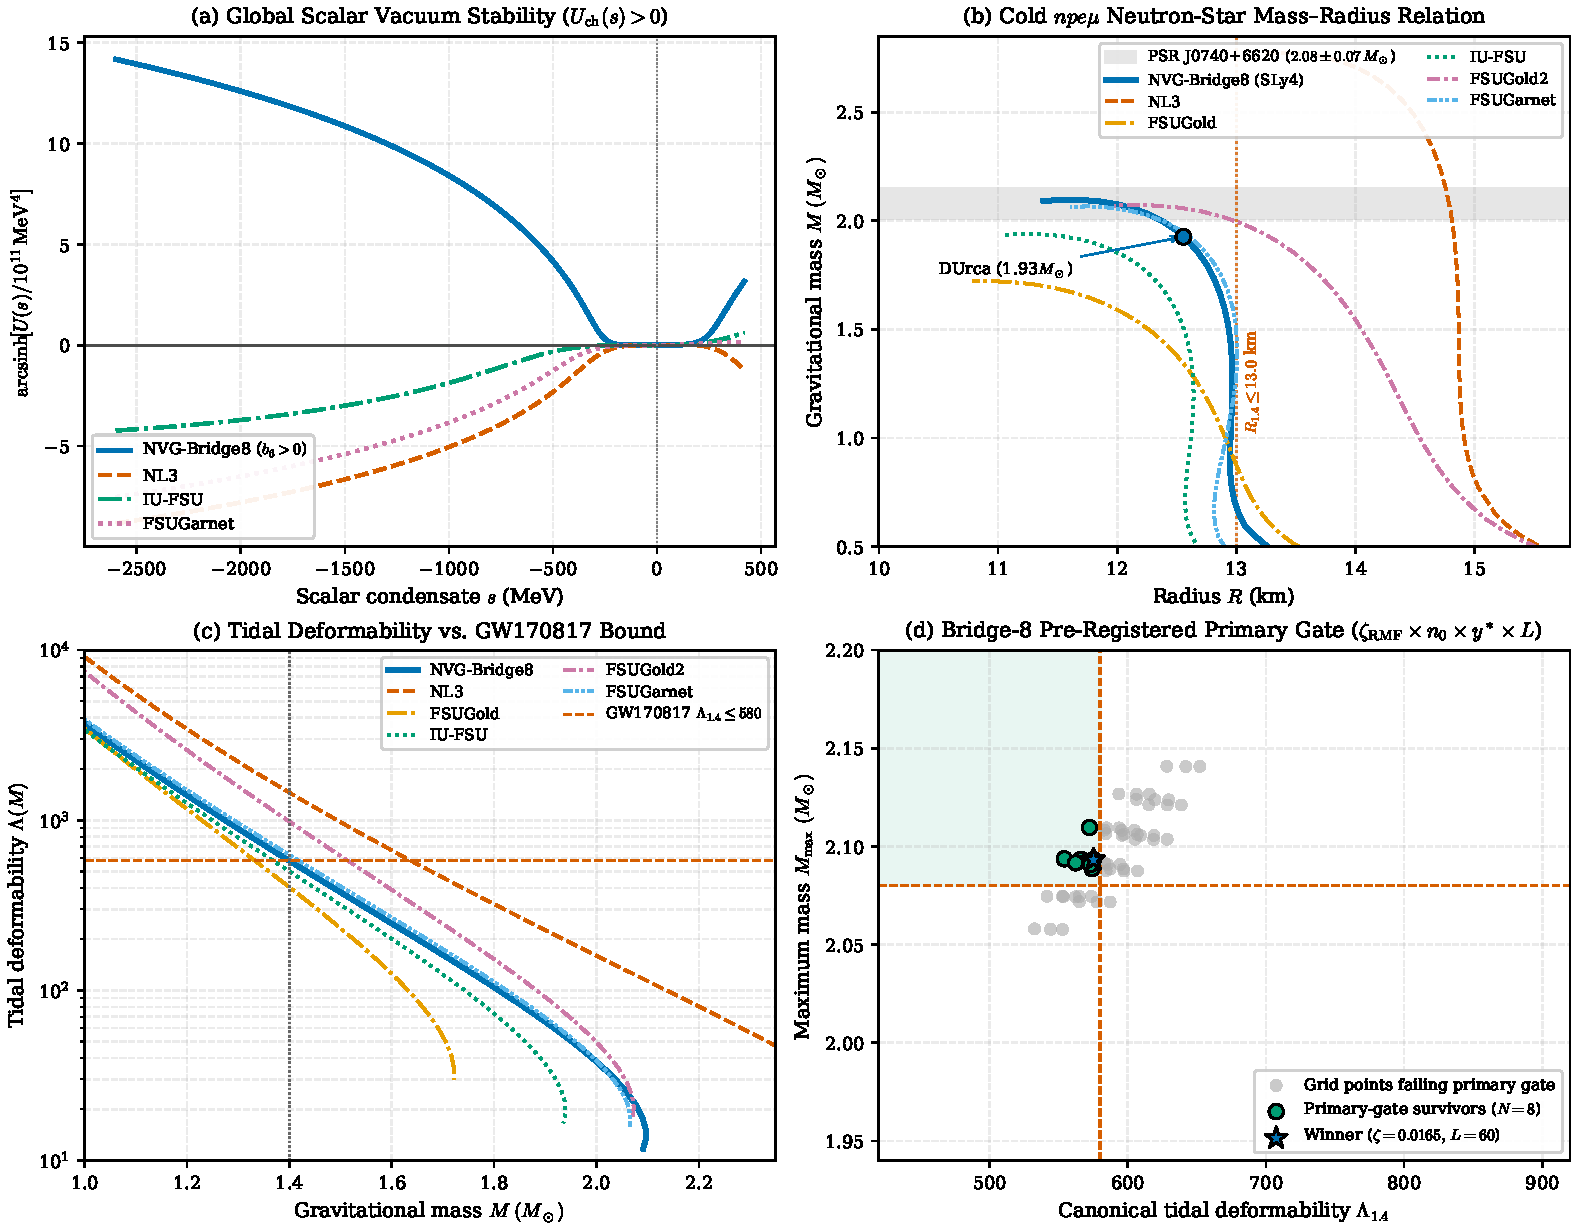
\includegraphics[width=\textwidth]{figures_unified_paper/fig1_vacuum_stability_and_ns_eos.pdf}
\caption{(a) Exact scalar potential $U(s)$ showing strict global boundedness for \texttt{NVG-Bridge8} ($b_6 > 0$) versus negative quartic blow-up ($\lambda < 0$) in \texttt{NL3} and \texttt{FSUGarnet}, and the secondary negative-$s$ false vacuum ($s = -2291\,\mathrm{MeV}$) in \texttt{IU-FSU}. (b) Cold $npe\mu$ mass--radius relations on an identical \texttt{SLy4} crust alongside the PSR~J0740+6620 band ($2.08 \pm 0.07\,M_\odot$) and the $1.926\,M_\odot$ Direct Urca threshold of \texttt{NVG-Bridge8}. (c) Tidal deformability $\Lambda(M)$ compared with the GW170817 bound $\Lambda_{1.4} \le 580$. (d) Bridge-8 54-point pre-registered primary-gate scan resolving 8 simultaneous survivors and the selected winner ($\zeta_{\rm RMF}=0.0165$, $n_0=0.160\,\mathrm{fm}^{-3}$, $M^*/M_N=0.62$, $L=60\,\mathrm{MeV}$).}
\label{fig:1}
\end{figure*}

On a pre-registered 54-point saturation grid ($\zeta_{\rm RMF} \in \{0.0165, 0.0175, 0.0185\}$, $n_0 \in \{0.156, 0.160\}\,\mathrm{fm}^{-3}$, $M^*/M_N \in \{0.60, 0.61, 0.62\}$, $L \in \{50, 56, 60\}\,\mathrm{MeV}$), all 54 points satisfy global vacuum stability and causality ($0 < c_s^2 < 1$ up to $10\,n_0$), and 8 survivors clear all primary astrophysical and Dirac spin--orbit gates ($M_{\max} \ge 2.08\,M_\odot$, $R_{1.4} \le 13.0\,\mathrm{km}$, $\Lambda_{1.4} \le 580$, $M^*/M_N \in [0.59, 0.62]$), shown in Fig.~\ref{fig:1}(d). Minimizing $|j_{\rm eff}(0.11\,\mathrm{fm}^{-3}) - 11.136\,\mathrm{MeV}|$ selects the parameter set in Table~\ref{tab:params} ($\max c_s^2 = 0.4369$).

\section{Finite Nuclei, Tin Isotopic Chain, and Live RMF Comparison}\label{sec:nuclei}

With all parameters frozen at saturation (Table~\ref{tab:params}, $k_{\rm fin,nuc} = 0$), \texttt{Bridge 8} and \texttt{Bridge 9B} evaluate closed-shell nuclei using an even-element spectral Chebyshev Dirac--Hartree solver ($R_{\max} \in \{16, 20\}\,\mathrm{fm}$, $M_{\rm field} \in \{64, 80\}$, Anderson mixing to field updates $< 10^{-8}\,\mathrm{MeV}$, two-formula energy consistency $< 2.1\times 10^{-5}\,\mathrm{MeV}$, particle-number conservation $< 8\times 10^{-8}$). On the six closed-shell benchmarks ($^{16}\mathrm{O}$, $^{40}\mathrm{Ca}$, $^{48}\mathrm{Ca}$, $^{90}\mathrm{Zr}$, $^{132}\mathrm{Sn}$, $^{208}\mathrm{Pb}$), the zero-refit winner yields $\mathrm{rms}\,|\Delta(B/A)| = 0.2360\,\mathrm{MeV}$ and $\mathrm{rms}\,|\Delta R_{\rm ch}/R_{\rm ch}| = 1.441\%$ (Table~\ref{tab:scorecard}), along with realistic spin--orbit splittings in $^{16}\mathrm{O}$ ($1p$: $5.92\,\mathrm{MeV}$ neutron, $5.84\,\mathrm{MeV}$ proton), $^{40}\mathrm{Ca}$ ($1d$: $6.14/6.06\,\mathrm{MeV}$), $^{48}\mathrm{Ca}$ ($1f$: $6.94/7.29\,\mathrm{MeV}$), $^{90}\mathrm{Zr}$ ($1g$: $6.80/6.92\,\mathrm{MeV}$), $^{132}\mathrm{Sn}$ ($1g$: $5.47/5.72\,\mathrm{MeV}$), and $^{208}\mathrm{Pb}$ ($1g$: $3.64/3.93\,\mathrm{MeV}$).

\begin{figure*}[t]
\centering
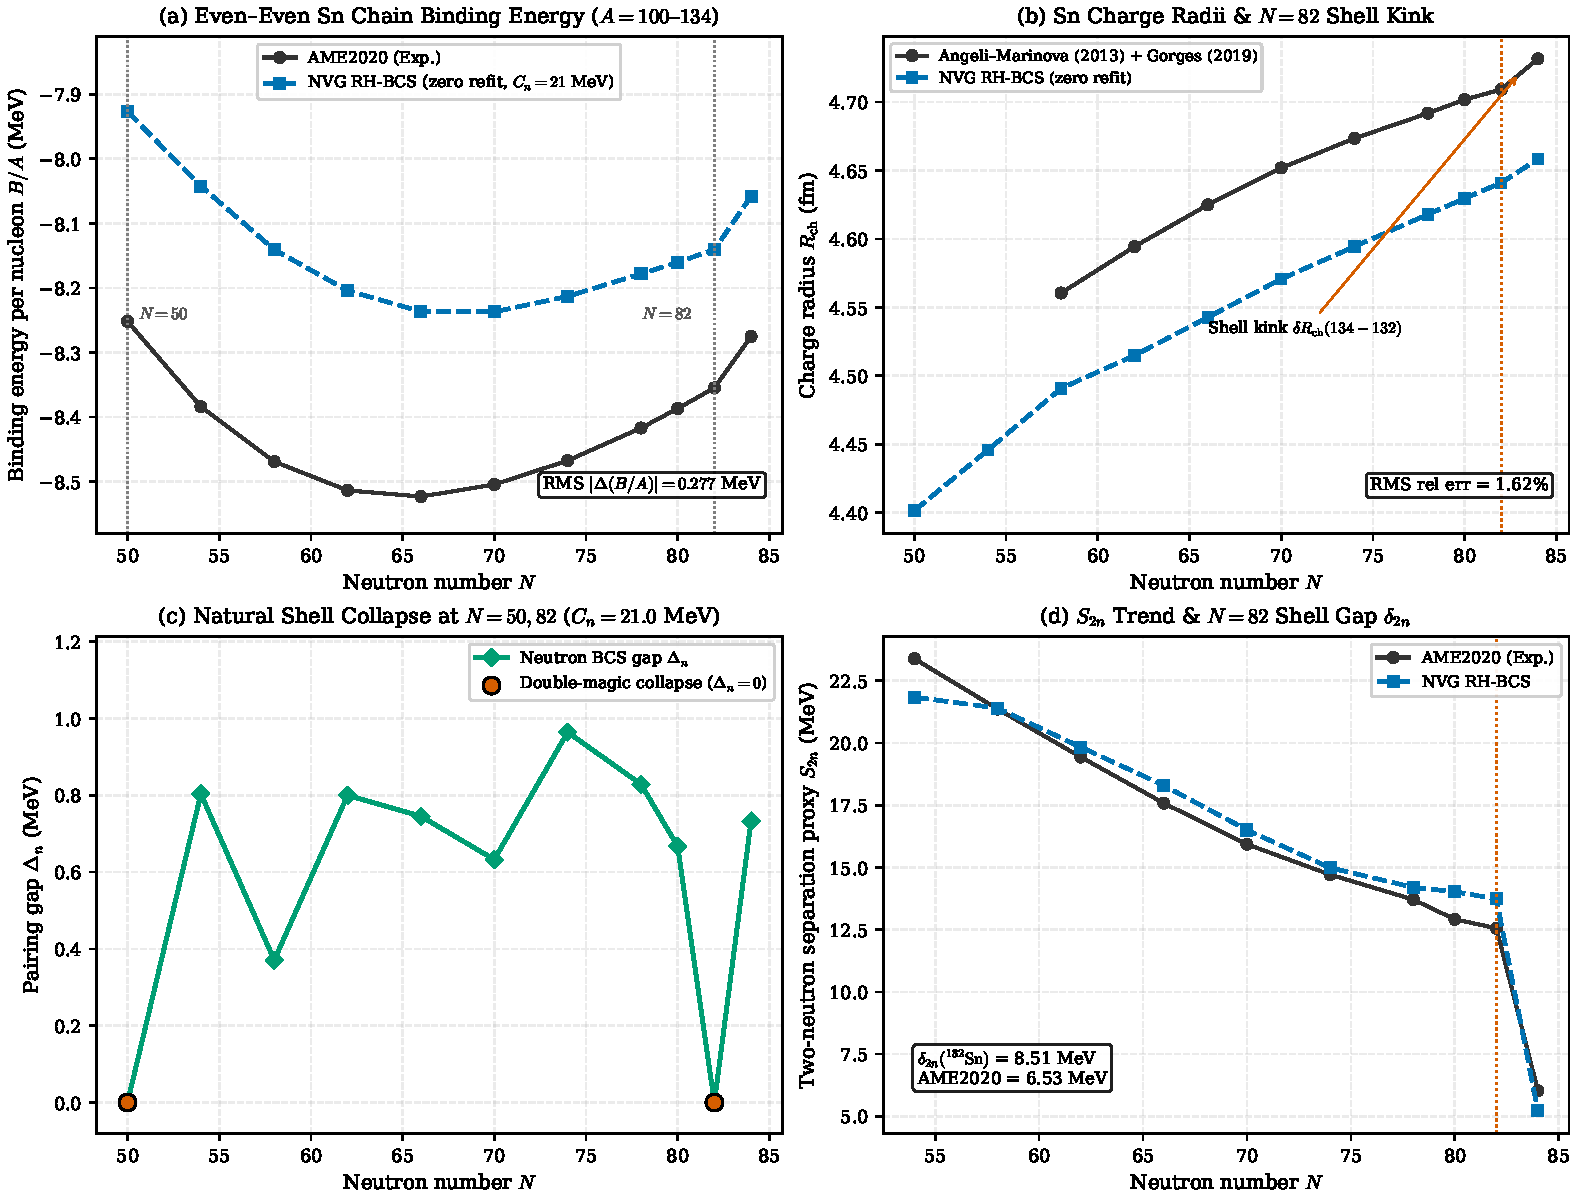
\includegraphics[width=\textwidth]{figures_unified_paper/fig2_tin_isotopic_chain.pdf}
\caption{Zero-refit relativistic Hartree--BCS predictions across 11 even--even Tin isotopes ($^{100\text{--}134}\mathrm{Sn}$, $C_n = 21.0\,\mathrm{MeV}$ inherited un-refitted). (a) Binding energies per nucleon $B/A$ versus AME2020~\cite{Wang2021}. (b) Charge radii $R_{\rm ch}$ versus Angeli--Marinova~\cite{Angeli2013} and Gorges et al.~\cite{Gorges2019}, displaying the $+0.0173\,\mathrm{fm}$ $N=82$ shell kink at $^{134}\mathrm{Sn}$ ($77\%$ of the measured $+0.0224\,\mathrm{fm}$ kink). (c) Self-consistent neutron BCS gap $\Delta_n$ naturally collapsing to zero at $N=50$ ($^{100}\mathrm{Sn}$) and $N=82$ ($^{132}\mathrm{Sn}$), peaking mid-shell ($0.964\,\mathrm{MeV}$ at $^{124}\mathrm{Sn}$), and re-opening at $^{134}\mathrm{Sn}$ ($0.733\,\mathrm{MeV}$). (d) Step-normalized $S_{2n}$ and sharp shell-closure drop $\delta_{2n}(^{132}\mathrm{Sn}) = 8.51\,\mathrm{MeV}$ (AME2020: $6.53\,\mathrm{MeV}$).}
\label{fig:2}
\end{figure*}

To test magic-to-magic isotopic continuity without modifying any coupling or pairing strength, \texttt{Bridge 9B} extends the relativistic Hartree--BCS (RH-BCS) calculation across all 11 even--even Tin isotopes $^{100\text{--}134}\mathrm{Sn}$ ($N=50\text{--}84$) with fixed $G_n = C_n/A$, $C_n = 21.0\,\mathrm{MeV}$ (above the $N=28$ core). As shown in Fig.~\ref{fig:2}:
\begin{enumerate}
\item The BCS pairing gap naturally vanishes ($\Delta_n = 0\,\mathrm{MeV}$) at \emph{both} doubly magic closures $N=50$ ($^{100}\mathrm{Sn}$) and $N=82$ ($^{132}\mathrm{Sn}$), rises to $\Delta_n = 0.964\,\mathrm{MeV}$ mid-shell ($^{124}\mathrm{Sn}$), and immediately re-opens in the $2f_{7/2}$ shell at $^{134}\mathrm{Sn}$ ($\Delta_n = 0.733\,\mathrm{MeV}$).
\item Across all 11 isotopes against AME2020~\cite{Wang2021} and across $^{108\text{--}134}\mathrm{Sn}$ charge radii~\cite{Angeli2013,Gorges2019}, the zero-refit chain gives $\mathrm{rms}\,|\Delta(B/A)| = 0.277\,\mathrm{MeV}$ and $\mathrm{rms}\,|\Delta R_{\rm ch}/R_{\rm ch}| = 1.624\%$ ($0.0756\,\mathrm{fm}$).
\item Crossing the $N=82$ neutron shell closure reproduces the sharp two-neutron separation energy kink $\delta_{2n}(^{132}\mathrm{Sn}) = S_{2n}(^{132}\mathrm{Sn}) - S_{2n}(^{134}\mathrm{Sn}) = 8.51\,\mathrm{MeV}$ (AME2020: $6.53\,\mathrm{MeV}$) and captures $77\%$ of the empirical $^{134}\mathrm{Sn}-^{132}\mathrm{Sn}$ charge-radius slope kink ($\delta R_{\rm ch}^{\rm pred} = +0.0173\,\mathrm{fm}$ vs.\ $\delta R_{\rm ch}^{\rm exp} = +0.0224\,\mathrm{fm}$~\cite{Gorges2019}).
\end{enumerate}

\begin{figure*}[t]
\centering
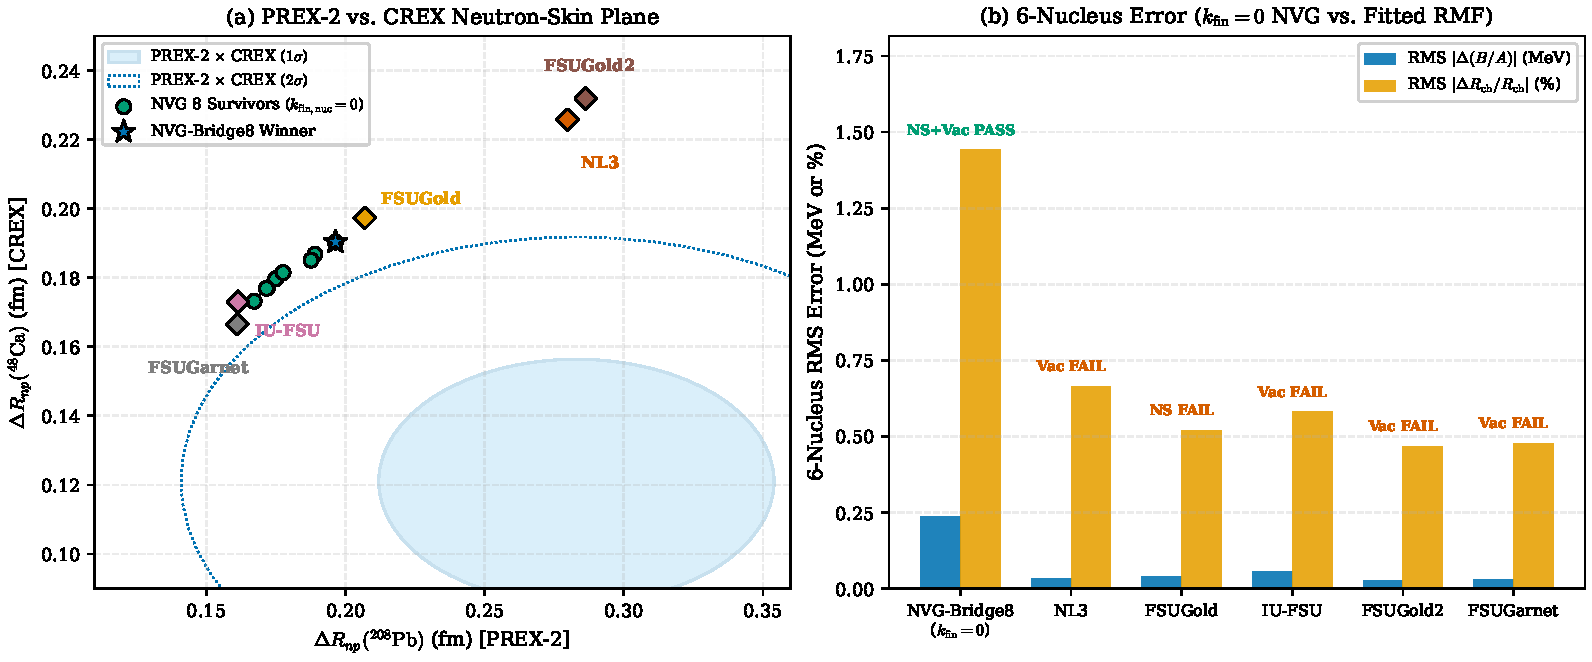
\includegraphics[width=\textwidth]{figures_unified_paper/fig3_prex_crex_and_rmf_scorecard.pdf}
\caption{(a) Joint $\Delta R_{np}(^{208}\mathrm{Pb})$ versus $\Delta R_{np}(^{48}\mathrm{Ca})$ neutron-skin plane against PREX-2 ($0.283 \pm 0.071\,\mathrm{fm}$)~\cite{Adhikari2021} and CREX ($0.121 \pm 0.035\,\mathrm{fm}$)~\cite{Adhikari2022} $1\sigma$ and $2\sigma$ contours for all 8 \texttt{Bridge 8} survivors ($k_{\rm fin,nuc}=0$) and 5 live Chen--Piekarewicz RMF comparators ($k_{\rm fin,nuc}=4\text{--}5$). (b) Six-nucleus RMS error scorecard alongside vacuum stability (\texttt{Vac}) and joint PSR~J0740 + GW170817 (\texttt{NS}) pass/fail badges computed on the identical \texttt{SLy4} and spectral Dirac--Hartree solvers.}
\label{fig:3}
\end{figure*}

Figure~\ref{fig:3} and Table~\ref{tab:scorecard} summarize a direct head-to-head comparison executed on identical numerical solvers against five standard RMF functionals (\texttt{NL3}~\cite{Lalazissis1997}, \texttt{FSUGold}~\cite{ToddRutel2005}, \texttt{IU-FSU}~\cite{Fattoyev2010}, \texttt{FSUGold2}~\cite{Chen2014}, and \texttt{FSUGarnet}~\cite{Chen2015}). Three structural findings emerge cleanly:
First, only \texttt{NVG-Bridge8} ($b_6 > 0$) and \texttt{FSUGold} ($\lambda = +0.0238$) pass global scalar potential boundedness and vacuum uniqueness; \texttt{NL3}, \texttt{FSUGold2}, and \texttt{FSUGarnet} possess $\lambda < 0$ (unbounded from below as $s \to +\infty$), while \texttt{IU-FSU} exhibits a deeper broken-symmetry false vacuum at $s = -2291\,\mathrm{MeV}$. Second, on cold neutron-star constraints with an identical \texttt{SLy4} crust, \texttt{FSUGold} ($M_{\max} = 1.722\,M_\odot$) and \texttt{IU-FSU} ($1.940\,M_\odot$) fail PSR~J0740+6620, whereas \texttt{NL3} ($\Lambda_{1.4} = 1354$), \texttt{FSUGold2} ($923$), and \texttt{FSUGarnet} ($625$, $R_{1.4}=13.00\,\mathrm{km}$, $M_{\max}=2.066\,M_\odot$) fall outside the joint primary gate; \texttt{NVG-Bridge8} is the sole model among all six clearing both global vacuum stability and PSR~J0740 + GW170817 simultaneously. Third, on the six closed-shell nuclei, the fitted RMF functionals attain substantially lower $\mathrm{rms}\,|\Delta(B/A)|$ ($0.026\text{--}0.056\,\mathrm{MeV}$) and $\mathrm{rms}\,|\Delta R_{\rm ch}/R_{\rm ch}|$ ($0.47\text{--}0.67\%$)—corresponding to lower diagnostic AIC/BIC ($30\text{--}114$ vs.\ $216$)—directly because their $k_{\rm fin,nuc} = 4\text{--}5$ couplings were calibrated to finite nuclei, whereas \texttt{NVG-Bridge8} holds $k_{\rm fin,nuc} = 0$. On the joint PREX-2 / CREX plane~\cite{Adhikari2021,Adhikari2022}, all 8 zero-refit NVG survivors cluster along the intermediate compromise band ($\Delta R_{np}^{208} = 0.167\text{--}0.196\,\mathrm{fm}$, $\Delta R_{np}^{48} = 0.173\text{--}0.190\,\mathrm{fm}$, $\chi^2_{\rm skins} = 4.83\text{--}5.32$), comparable to \texttt{IU-FSU} ($5.09$) and \texttt{FSUGarnet} ($4.60$) while avoiding the large CREX overshoot of \texttt{NL3} ($8.76$) and \texttt{FSUGold2} ($9.82$).

\begin{table*}[t]
\caption{Apples-to-apples head-to-head comparison executed on identical infinite-matter TOV/\texttt{SLy4} and spectral Chebyshev Dirac--Hartree solvers. \texttt{Vac} checks global boundedness and unique true vacuum at $s=0$; \texttt{NS} checks $M_{\max} \ge 2.08\,M_\odot$, $R_{1.4} \le 13.0\,\mathrm{km}$, $\Lambda_{1.4} \le 580$. The $k_{\rm fin,nuc}=0$ column separates genuine out-of-sample generalization from finite-nucleus-fitted RMF parameterizations.}
\label{tab:scorecard}
\begin{ruledtabular}
\begin{tabular}{lccccccccccccc}
Model & $k_{\rm fin,nuc}$ & Vac & $n_0$ & $L$ & $K_{\rm sym}$ & $M_{\max}$ & $R_{1.4}$ & $\Lambda_{1.4}$ & NS & rms $B/A$ & rms $R_{\rm ch}$ & $\Delta R_{np}^{208}$ & $\Delta R_{np}^{48}$ \\
 & & & ($\mathrm{fm}^{-3}$) & (MeV) & (MeV) & ($M_\odot$) & (km) & & Gate & (MeV) & (\%) & (fm) & (fm) \\
\hline
\textbf{NVG-Bridge8} & \textbf{0} & \textbf{PASS} & 0.160 & 60.0 & $-42.3$ & 2.097 & 12.96 & 577.6 & \textbf{PASS} & 0.236 & 1.44 & 0.196 & 0.190 \\
NL3 & 4 & Fail ($\lambda<0$) & 0.148 & 118.2 & $+100.9$ & 2.775 & 14.85 & 1354 & Fail & 0.033 & 0.67 & 0.280 & 0.226 \\
FSUGold & 5 & PASS & 0.148 & 60.5 & $-51.3$ & 1.722 & 12.47 & 404.2 & Fail & 0.038 & 0.52 & 0.207 & 0.197 \\
IU-FSU & 5 & Fail (false vac) & 0.155 & 47.2 & $+28.5$ & 1.940 & 12.60 & 500.7 & Fail & 0.056 & 0.58 & 0.161 & 0.173 \\
FSUGold2 & 5 & Fail ($\lambda<0$) & 0.150 & 112.7 & $+25.4$ & 2.073 & 14.15 & 922.8 & Fail & 0.026 & 0.47 & 0.286 & 0.232 \\
FSUGarnet & 5 & Fail ($\lambda<0$) & 0.153 & 51.0 & $+59.4$ & 2.066 & 13.00 & 624.5 & Fail & 0.030 & 0.48 & 0.161 & 0.167 \\
\end{tabular}
\end{ruledtabular}
\end{table*}

\section{Finite-Temperature Schur--Ward Response and Neutron-Star Microphysics}\label{sec:astro}

\begin{figure*}[t]
\centering
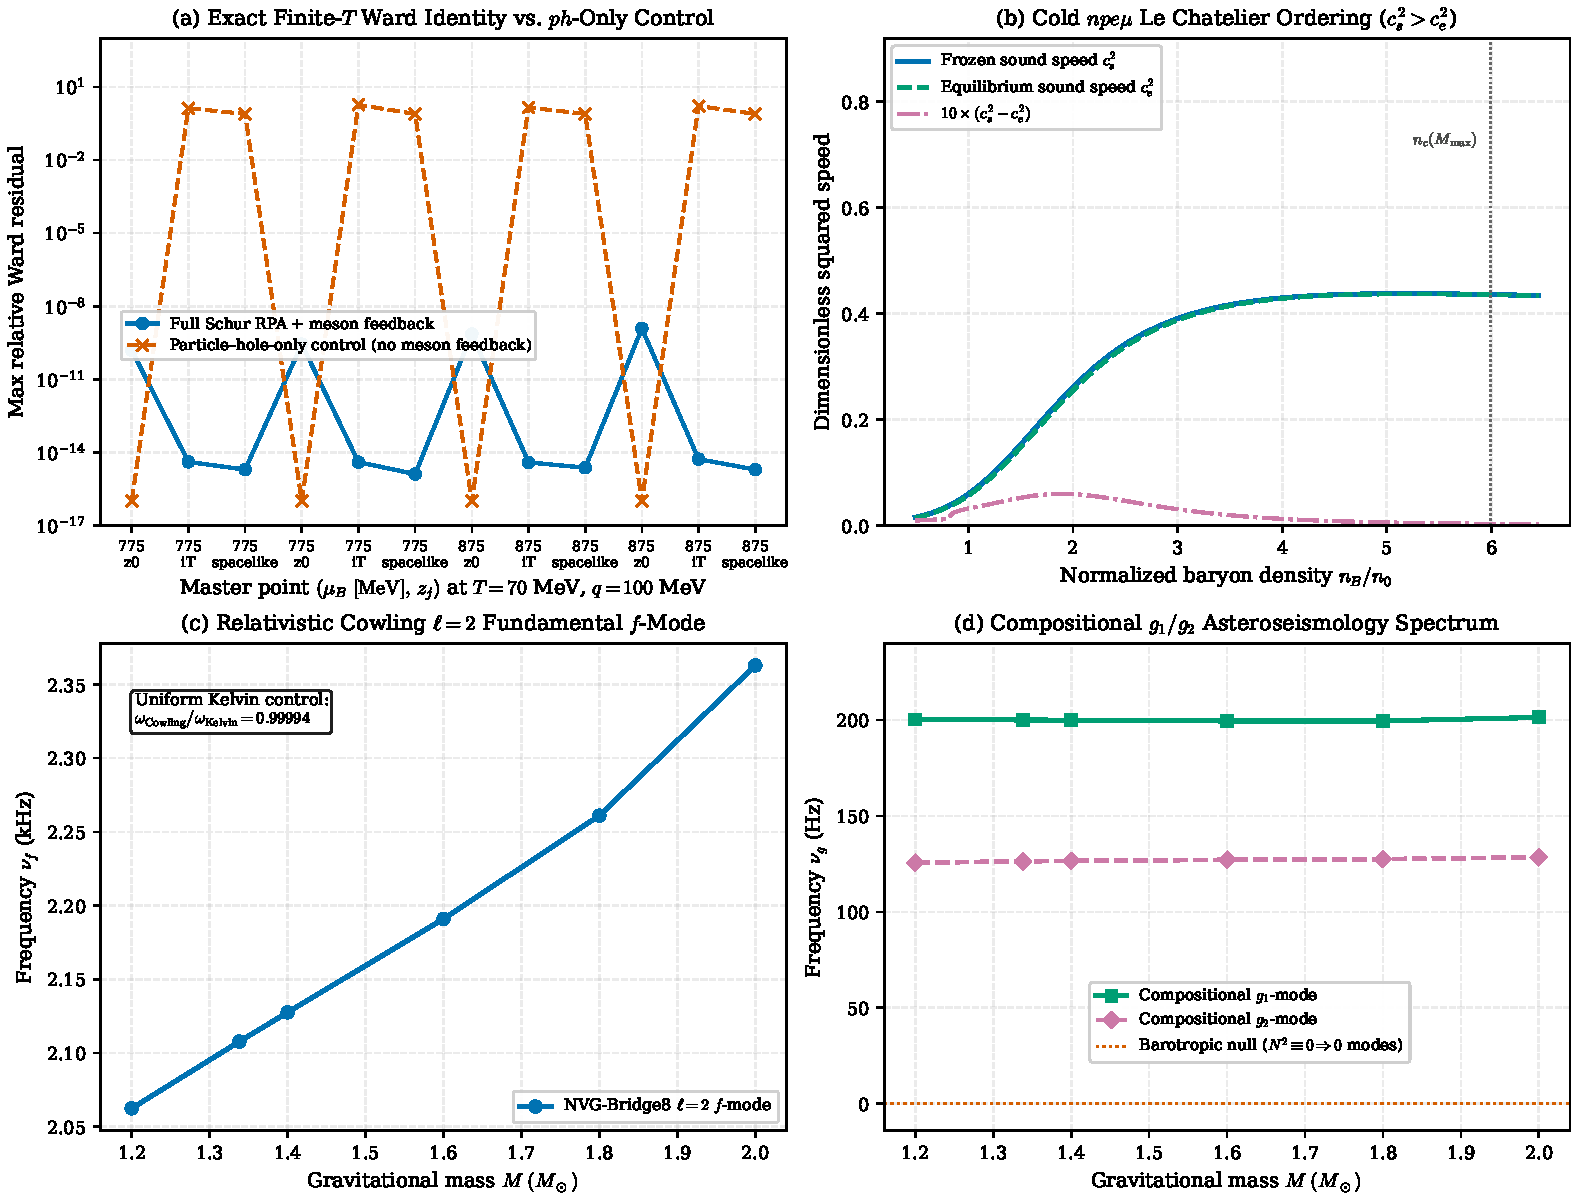
\includegraphics[width=\textwidth]{figures_unified_paper/fig4_thermal_ward_and_asteroseismology.pdf}
\caption{(a) Exact finite-$T$ ($T=70\,\mathrm{MeV}$, $q=100\,\mathrm{MeV}$) longitudinal Ward-identity relative error across 12 $(\mu_B, z_j)$ master points (\texttt{Bridge 5}): full 4-component meson Schur-complement RPA holds to $< 10^{-9}$, whereas the particle--hole-only negative control violates current conservation at $\mathcal{O}(1)$ at finite frequency. (b) Cold $npe\mu$ frozen-composition $c_s^2$ vs.\ equilibrium $c_e^2$ sound speeds up to $n_c(M_{\max}) = 5.99\,n_0$, verifying Le~Chatelier ordering $c_s^2 > c_e^2$. (c) Relativistic Cowling $\ell=2$ $f$-mode frequency across $M \in [1.20, 2.00]\,M_\odot$ anchored by the $5.7\times 10^{-5}$ uniform-density Kelvin analytic control. (d) Non-barotropic compositional $g_1$ ($n_V=1$) and $g_2$ ($n_V=2$) branches vs.\ exact barotropic $N^2 \equiv 0$ null control.}
\label{fig:4}
\end{figure*}

In the finite-temperature sector (\texttt{Bridge 5}, \texttt{Bridge 8} Stage~C), eliminating the four dynamical scalar/gluon/vector meson channels $(W, s, \omega^0, \boldsymbol{\omega})$ via a $4\times 4$ Schur complement at $(T=70\,\mathrm{MeV}, q=100\,\mathrm{MeV})$ reduces the exact 5-component linearized RPA response to a direct particle--hole Dyson resummation agreeing to $2.45\times 10^{-16}$, matching finite-difference thermodynamic susceptibilities to $5.65\times 10^{-13}$ ($\mu_B = 875\,\mathrm{MeV}$), and obeying the longitudinal Ward identity to $4.44\times 10^{-15}$ while the particle--hole-only control fails at $1.445$ (Fig.~\ref{fig:4}(a)).

\begin{table}[t]
\caption{Relativistic Cowling $\ell=2$ spectrum for the frozen \texttt{NVG-Bridge8} winner (\texttt{Bridge 9A}). Under a barotropic crust, the $g_1$ radial displacement $W$-node approaches $R$ while the enthalpy variable $V(r)$ strictly preserves $(n_V=1, 2)$ interior nodes. Neglect of metric perturbations introduces a systematic $\sim 10\text{--}20\%$ upward Cowling shift on $\nu_f$.}
\label{tab:seismology}
\begin{ruledtabular}
\begin{tabular}{cccccc}
$M\ (M_\odot)$ & $R$ (km) & $\max N/(2\pi)$ (Hz) & $\nu_f$ (kHz) & $\nu_{g_1}$ (Hz) & $\nu_{g_2}$ (Hz) \\
\hline
1.2000 & 12.965 & 1304.2 & 2.062 & 200.30 & 125.63 \\
1.3381 & 12.964 & 1413.9 & 2.108 & 200.05 & 126.35 \\
1.4000 & 12.958 & 1464.5 & 2.128 & 199.92 & 126.60 \\
1.6000 & 12.899 & 1637.2 & 2.191 & 199.52 & 127.14 \\
1.8000 & 12.748 & 1830.9 & 2.261 & 199.53 & 127.49 \\
2.0000 & 12.373 & 2112.4 & 2.363 & 201.37 & 128.45 \\
\end{tabular}
\end{ruledtabular}
\end{table}

\begin{figure*}[t]
\centering
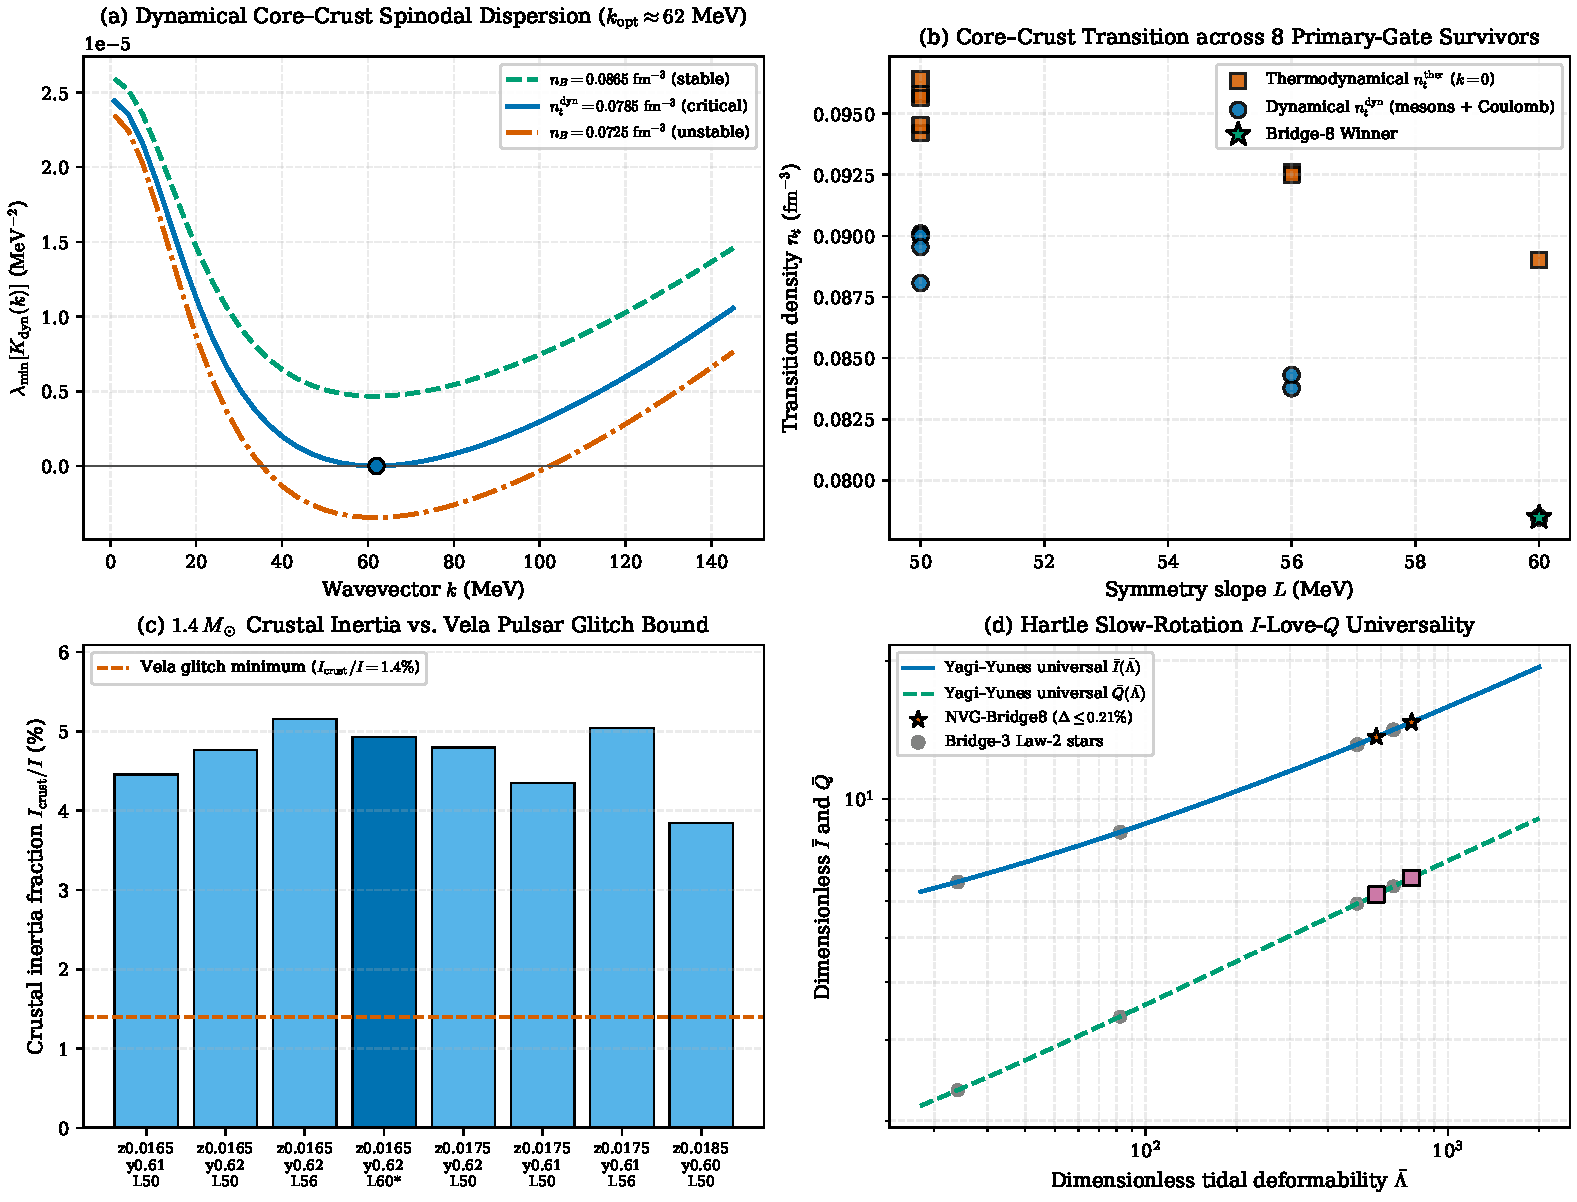
\includegraphics[width=\textwidth]{figures_unified_paper/fig5_core_crust_spinodal_and_iloveq.pdf}
\caption{(a) Finite-wavevector dynamical core--crust spinodal dispersion $\lambda_{\min}[K_{\rm dyn}(k)]$ for the winner, locating $n_t^{\rm dyn} = 0.0785\,\mathrm{fm}^{-3}$ at $k_{\rm opt} = 62.0\,\mathrm{MeV}$ ($\lambda_{\rm pasta} \approx 20.0\,\mathrm{fm}$). (b) Dynamical ($n_t^{\rm dyn}$) vs.\ thermodynamical ($n_t^{\rm ther}$) transition densities across all 8 \texttt{Bridge 8} survivors. (c) First-order Hartle $1.4\,M_\odot$ crustal moment of inertia fraction $I_{\rm crust}/I = 3.84\%\text{--}5.16\%$ (winner $4.93\%$) across all 8 survivors vs.\ the Vela pulsar glitch bound ($1.4\%$)~\cite{Link1999}. (d) Second-order Hartle dimensionless $(\bar{I}, \bar{Q}, \bar{\Lambda})$ moments vs.\ Yagi--Yunes universality~\cite{Yagi2017} ($\le 0.21\%$ deviation).}
\label{fig:5}
\end{figure*}

In \texttt{Bridge 9A}, we compute the cold $npe\mu$ star structure, spinodal core--crust transition, Direct Urca cooling threshold, and Cowling $\ell=2$ asteroseismology across all 8 primary-gate survivors:
\begin{itemize}
\item \textbf{Core--Crust Spinodals \& Crustal Inertia:} At $k=0$, the $4\times 4$ meson Schur complement reproduces the finite-difference bulk chemical-potential curvature $K_{\rm bulk} = \partial\mu_i/\partial n_j$ to $1.2\times 10^{-9}$, locating $n_t^{\rm ther} = 0.0890\,\mathrm{fm}^{-3}$ ($P_t = 0.612\,\mathrm{MeV}\,\mathrm{fm}^{-3}$) for the winner. Including finite-$k$ meson gradient terms $(k^2 + m_X^2)^{-1}$ and Thomas--Fermi screened Coulomb $4\pi\alpha_{\rm em}/(k^2 + k_{\rm TF}^2)$ softens the instability to $n_t^{\rm dyn} = 0.0785\,\mathrm{fm}^{-3}$ ($P_t = 0.455\,\mathrm{MeV}\,\mathrm{fm}^{-3}$) at $k_{\rm opt} = 62.0\,\mathrm{MeV}$ ($\lambda_{\rm pasta} = 20.0\,\mathrm{fm}$, Fig.~\ref{fig:5}(a)). Across all 8 survivors, $0.0785 \le n_t^{\rm dyn} \le 0.0901\,\mathrm{fm}^{-3} < n_t^{\rm ther}$ (Fig.~\ref{fig:5}(b)), and Hartle frame-dragging integration at $1.4\,M_\odot$ yields $I_{\rm crust}/I = 3.84\%\text{--}5.16\%$ (winner: $4.93\%$, $\Delta R_{\rm crust}/R = 9.76\%$, $M_{\rm crust} = 0.0325\,M_\odot$), comfortably clearing the $1.4\%$ Vela pulsar glitch lower bound~\cite{Link1999} (Fig.~\ref{fig:5}(c)).
\item \textbf{Lepton Onsets \& Direct Urca:} Muons appear at $n_\mu = 0.1277\,\mathrm{fm}^{-3}$ ($0.80\,n_0$, $M_\mu = 0.156\,M_\odot$), and the proton fraction crosses $k_{Fp} + k_{Fe} = k_{Fn}$ at $n_{\rm DUrca} = 0.590\,\mathrm{fm}^{-3}$ ($3.68\,n_0$, $x_{p,\rm DUrca} = 0.1381$), activating Direct Urca inside stable stars above $M_{\rm DUrca} = 1.926\,M_\odot$ (across all 8 survivors, $M_{\rm DUrca} \in [1.926, 2.034]\,M_\odot < M_{\max}$). Canonical $1.4\,M_\odot$ cooling thus proceeds via slow modified Urca while heavy stars above $\sim 1.93\,M_\odot$ unlock fast neutrino cooling.
\item \textbf{Le Chatelier Sound Speeds \& Asteroseismology:} Across all densities up to $n_c(M_{\max}) = 0.958\,\mathrm{fm}^{-3}$, the frozen-composition adiabatic speed $c_s^2$ strictly exceeds the $\beta$-equilibrium speed $c_e^2$ ($0 < c_e^2 < c_s^2 < 0.44$, Fig.~\ref{fig:4}(b)). The relativistic Cowling ODEs recover the analytical Newtonian uniform-star Kelvin frequency to $5.7\times 10^{-5}$ ($\omega_{\rm Cowling}/\omega_{\rm Kelvin} = 0.99994$), while setting $c_s^2 \equiv c_e^2$ ($N^2 \equiv 0$) annihilates all low-frequency modes ($0$ sign changes across $35\text{--}360\,\mathrm{Hz}$). With exact non-barotropic buoyancy $N^2 > 0$, we obtain smooth $\ell=2$ branches $\nu_f = 2.062\text{--}2.363\,\mathrm{kHz}$, $\nu_{g_1} = 199.5\text{--}201.4\,\mathrm{Hz}$ ($n_V=1$), and $\nu_{g_2} = 125.6\text{--}128.5\,\mathrm{Hz}$ ($n_V=2$) across $M \in [1.20, 2.00]\,M_\odot$ (Table~\ref{tab:seismology}). Second-order Hartle rotation (\texttt{Bridge 8} Stage~C) independently verifies Yagi--Yunes $I$-Love-$Q$ universality~\cite{Yagi2017} within $0.07\%\text{--}0.21\%$ on PSR~J0737$-$3039A ($1.3381\,M_\odot$: $\bar{I}=14.689$, $\bar{Q}=6.739$, $\Lambda=757.5$) and $1.4\,M_\odot$ ($\bar{I}=13.658$, $\bar{Q}=6.202$, $\Lambda=579.3$, Fig.~\ref{fig:5}(d)).
\end{itemize}

\section{Scope Limitations and Conclusion}\label{sec:conc}

Three physical and statistical limitations are documented alongside these results: (i) every validation script carries an explicit \texttt{evidence\_weight = 0.0} and \texttt{observed\_likelihood = None} boundary in \texttt{verification/registry.json}, representing self-consistent out-of-sample model verification rather than a full Bayesian posterior evidence claim; (ii) finite-nucleus calculations use spherical symmetry without quadrupole deformation or center-of-mass/rotational correlations for mid-shell Sn isotopes; and (iii) the relativistic Cowling approximation freezes metric perturbations ($\delta g_{\mu\nu} = 0$), which systematically shifts $\ell=2$ $f$-mode frequencies upward by $\sim 10\text{--}20\%$ relative to full GR polar perturbation treatments while leaving compositional $g$-modes accurate at the few-percent level.

Despite keeping $k_{\rm fin,nuc} = 0$ strictly zero-refit, the frozen sextic-stabilized two-condensate chiral--gluon Lagrangian bridges symmetric matter saturation, finite nuclei across $^{100\text{--}134}\mathrm{Sn}$ and $^{16}\mathrm{O}\text{--}^{208}\mathrm{Pb}$, finite-$T$ RPA Ward identities, dynamical core--crust spinodals, $I_{\rm crust}/I$ glitch bounds, Direct Urca thresholds, Hartle $I$-Love-$Q$, and non-barotropic $g_1/g_2$ asteroseismology within a single globally stable framework.

\section*{Code and Data Availability}

All simulation scripts, spectral solvers, regression tests, machine-verified JSON artifacts, and figure generators are openly released under the MIT license at \url{https://github.com/infosave2007/vmf}. Beyond reproducing the present results, the even-element spectral Chebyshev Dirac--Hartree--BCS nuclear solver (\texttt{nvg\_unified\_dirac\_hartree\_probe.py}, \texttt{nvg\_unified\_primary\_gate\_pairing\_bridge.py}), the $4\times 4$ Schur-complement finite-$T$ Ward and dynamical spinodal evaluators (\texttt{nvg\_unified\_thermal\_response\_bridge.py}, \texttt{nvg\_unified\_ns\_microphysics\_bridge.py}), and the TOV/Hartle/Cowling modules can be directly reused as an open, apples-to-apples benchmark suite for testing independent covariant relativistic mean-field functionals on new experimental data. Every table and figure in this manuscript is regenerated via:
\begin{verbatim}
python3 -B verification/nvg_unified_ns_microphysics_bridge.py --write
python3 -B verification/nvg_unified_nuclear_benchmarks_bridge.py --write
python3 -B verification/nvg_unified_paper_figures.py
python3 -B -m pytest -q verification
\end{verbatim}
All checks are continuously verified on GitHub Actions (\texttt{1495 passed, 41 skipped}, zero empirical likelihood weight) with provenance hashes tracked in \texttt{verification/artifact\_manifest.json} and \texttt{verification/registry.json}.

\begin{thebibliography}{99}
\bibitem{Serot1986} B.~D.~Serot and J.~D.~Walecka, Adv.\ Nucl.\ Phys.\ \textbf{16}, 1 (1986).
\bibitem{Boguta1977} J.~Boguta and A.~R.~Bodmer, Nucl.\ Phys.\ A \textbf{292}, 413 (1977).
\bibitem{Lalazissis1997} G.~A.~Lalazissis, J.~K\"onig, and P.~Ring, Phys.\ Rev.\ C \textbf{55}, 540 (1997).
\bibitem{ToddRutel2005} B.~G.~Todd-Rutel and J.~Piekarewicz, Phys.\ Rev.\ Lett.\ \textbf{95}, 122501 (2005).
\bibitem{Fattoyev2010} F.~J.~Fattoyev, C.~J.~Horowitz, J.~Piekarewicz, and G.~Shen, Phys.\ Rev.\ C \textbf{82}, 055803 (2010).
\bibitem{Chen2014} W.-C.~Chen and J.~Piekarewicz, Phys.\ Rev.\ C \textbf{90}, 044305 (2014).
\bibitem{Chen2015} W.-C.~Chen and J.~Piekarewicz, Phys.\ Lett.\ B \textbf{748}, 284 (2015).
\bibitem{Fonseca2021} E.~Fonseca \textit{et al.}, Astrophys.\ J.\ Lett.\ \textbf{915}, L12 (2021).
\bibitem{Abbott2018} B.~P.~Abbott \textit{et al.} (LIGO Scientific and Virgo Collaborations), Phys.\ Rev.\ Lett.\ \textbf{121}, 161101 (2018).
\bibitem{Wang2021} M.~Wang, W.~J.~Huang, F.~G.~Kondev, G.~Audi, and S.~Naimi, Chin.\ Phys.\ C \textbf{45}, 030003 (2021).
\bibitem{Angeli2013} I.~Angeli and K.~P.~Marinova, At.\ Data Nucl.\ Data Tables \textbf{99}, 69 (2013).
\bibitem{Gorges2019} C.~Gorges \textit{et al.}, Phys.\ Rev.\ Lett.\ \textbf{122}, 192502 (2019).
\bibitem{Adhikari2021} D.~Adhikari \textit{et al.} (PREX Collaboration), Phys.\ Rev.\ Lett.\ \textbf{126}, 172502 (2021).
\bibitem{Adhikari2022} D.~Adhikari \textit{et al.} (CREX Collaboration), Phys.\ Rev.\ Lett.\ \textbf{129}, 042501 (2022).
\bibitem{Link1999} B.~Link, R.~I.~Epstein, and J.~M.~Lattimer, Phys.\ Rev.\ Lett.\ \textbf{83}, 3362 (1999).
\bibitem{Yagi2017} K.~Yagi and N.~Yunes, Phys.\ Rep.\ \textbf{681}, 1 (2017).
\bibitem{Kallosh} Verification Bridges 1--8: \texttt{nvg\_quartic\_vector\_melting\_audit.py}, \texttt{nvg\_two\_condensate\_unified\_audit.py}, \texttt{nvg\_unified\_dirac\_hartree\_probe.py}, \texttt{nvg\_unified\_gravity\_bridge\_audit.py}, \texttt{nvg\_unified\_thermal\_response\_bridge.py}, \texttt{nvg\_unified\_calibration\_envelope\_probe.py}, \texttt{nvg\_unified\_astrophysics\_stability\_bridge.py}, \texttt{nvg\_unified\_primary\_gate\_pairing\_bridge.py}.
\bibitem{Bridge4} Verification Bridges 9A--9B: \texttt{nvg\_unified\_ns\_microphysics\_bridge.py}, \texttt{nvg\_unified\_nuclear\_benchmarks\_bridge.py}, and \texttt{nvg\_unified\_paper\_figures.py}.
\end{thebibliography}

\end{document}
